\documentclass{standalone}
\usepackage{tikz}
\usetikzlibrary{patterns, positioning}
\usepackage[sfdefault]{ClearSans} %% option 'sfdefault' activates Clear Sans as the default text font
\usepackage[T1]{fontenc}

\begin{document}
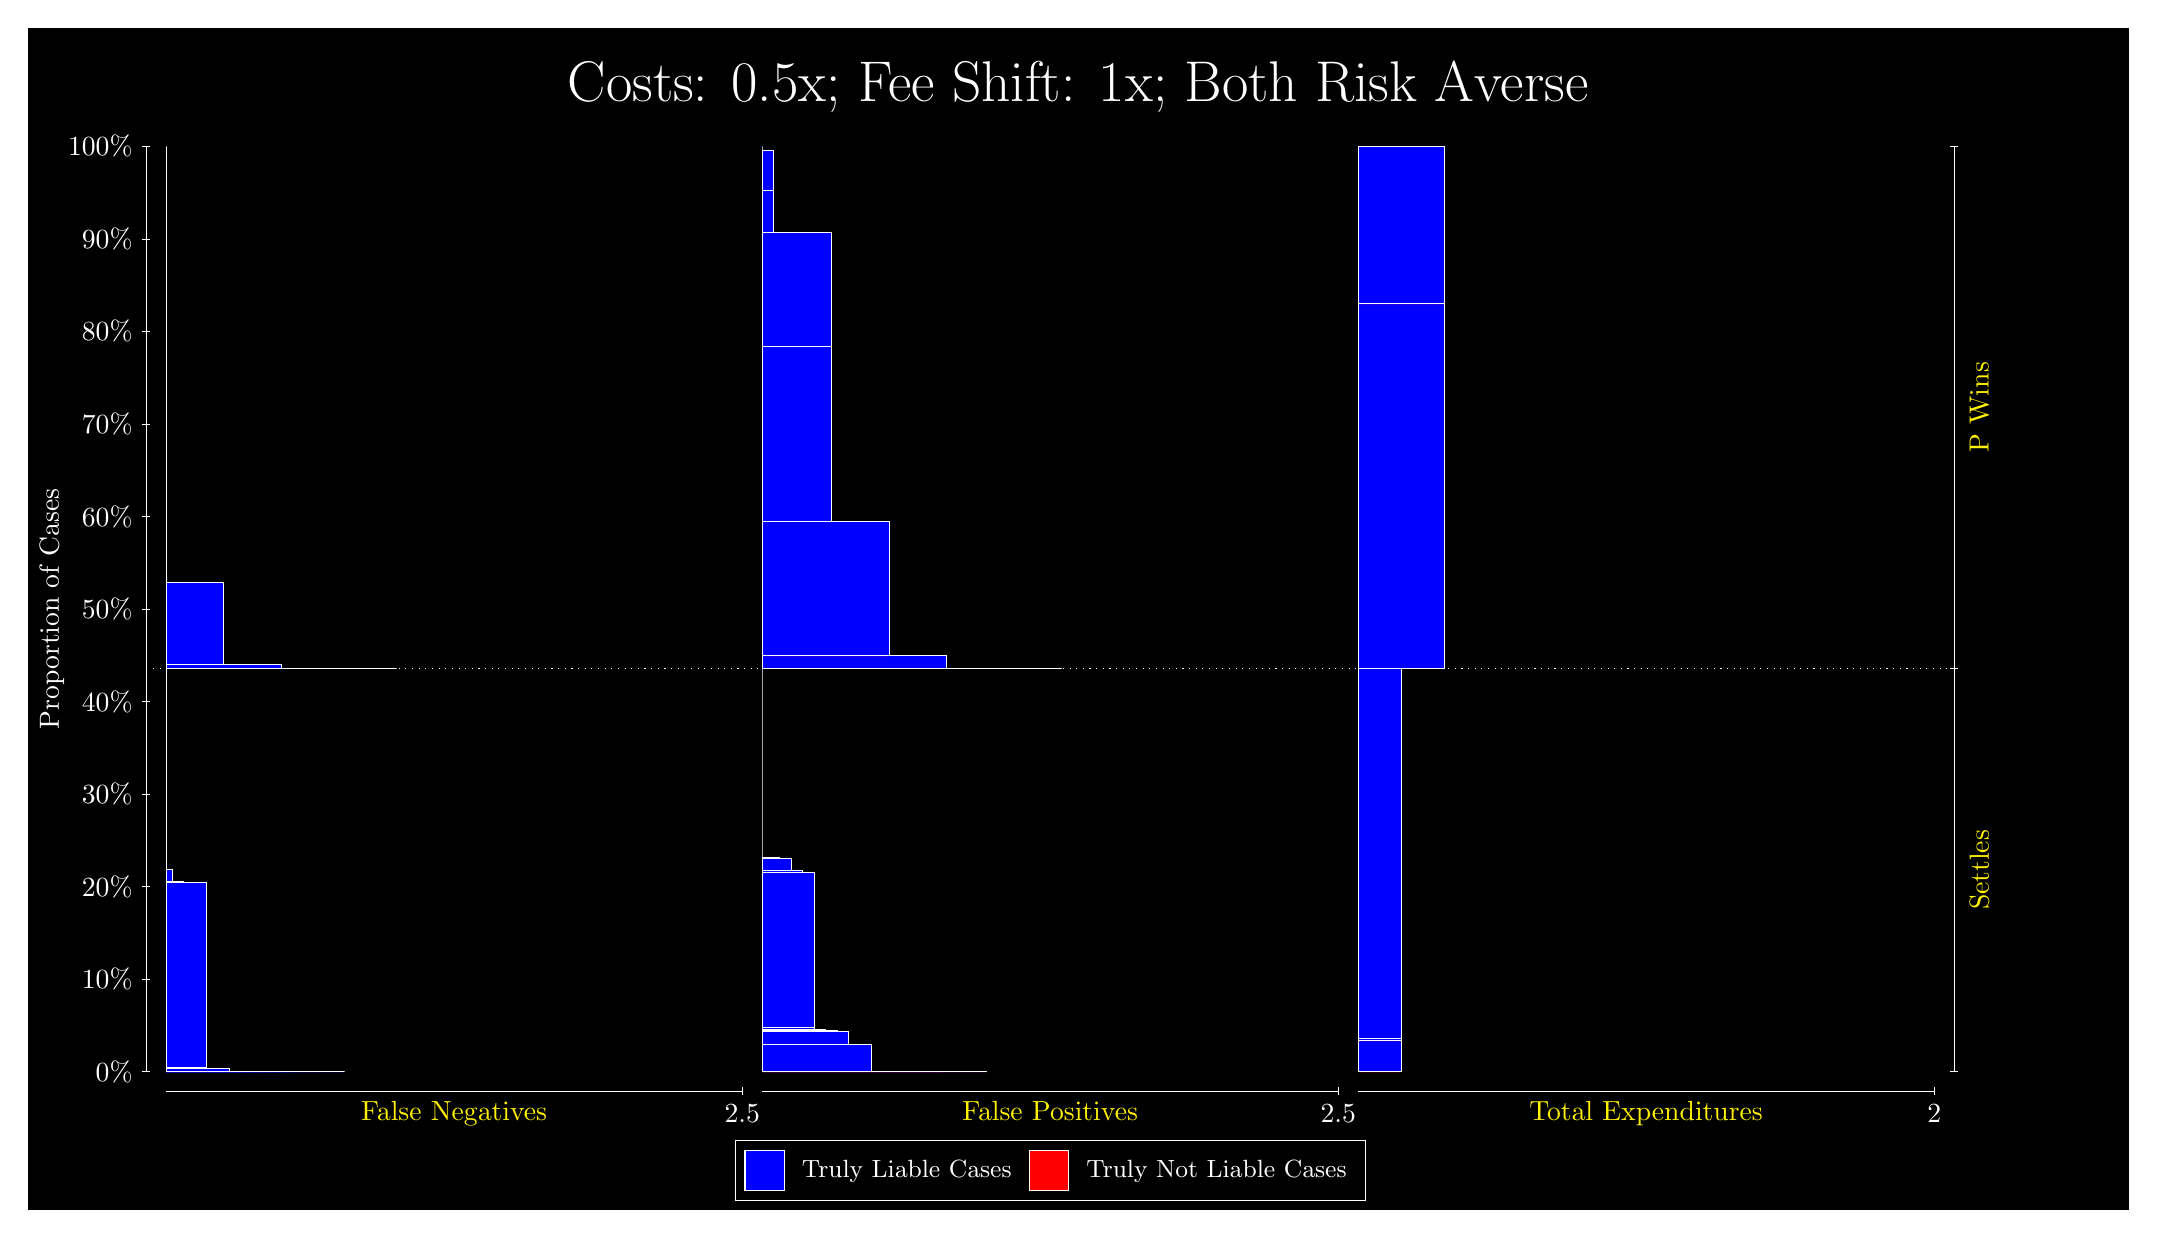
\begin{tikzpicture}
\draw[fill=black] (0,0) rectangle (26.667,15);
\draw[text=white] (0,13.5) rectangle (26.667,15) node[midway] {\huge Costs: 0.5x; Fee Shift: 1x; Both Risk Averse};
\draw[white, very thin] (1.5,1.75) -- (1.5,13.5);
\node[rotate=90, text=white, anchor=center] at (0.3, 7.625) {Proportion of Cases};
\draw[white, very thin] (1.45,1.75) -- (1.55,1.75);
\node[text=white, anchor=east] at (1.45, 1.75) {0\%};
\draw[white, very thin] (1.45,2.925) -- (1.55,2.925);
\node[text=white, anchor=east] at (1.45, 2.925) {10\%};
\draw[white, very thin] (1.45,4.1) -- (1.55,4.1);
\node[text=white, anchor=east] at (1.45, 4.1) {20\%};
\draw[white, very thin] (1.45,5.275) -- (1.55,5.275);
\node[text=white, anchor=east] at (1.45, 5.275) {30\%};
\draw[white, very thin] (1.45,6.45) -- (1.55,6.45);
\node[text=white, anchor=east] at (1.45, 6.45) {40\%};
\draw[white, very thin] (1.45,7.625) -- (1.55,7.625);
\node[text=white, anchor=east] at (1.45, 7.625) {50\%};
\draw[white, very thin] (1.45,8.8) -- (1.55,8.8);
\node[text=white, anchor=east] at (1.45, 8.8) {60\%};
\draw[white, very thin] (1.45,9.975) -- (1.55,9.975);
\node[text=white, anchor=east] at (1.45, 9.975) {70\%};
\draw[white, very thin] (1.45,11.15) -- (1.55,11.15);
\node[text=white, anchor=east] at (1.45, 11.15) {80\%};
\draw[white, very thin] (1.45,12.325) -- (1.55,12.325);
\node[text=white, anchor=east] at (1.45, 12.325) {90\%};
\draw[white, very thin] (1.45,13.5) -- (1.55,13.5);
\node[text=white, anchor=east] at (1.45, 13.5) {100\%};

\draw[white, very thin] (24.457,1.75) -- (24.457,13.5);
\draw[white, very thin] (24.407,1.75) -- (24.507,1.75);
\node[anchor=west] at (24.407, 1.75) {};
\draw[white, very thin] (24.407,6.8723) -- (24.507,6.8723);
\node[anchor=west] at (24.407, 6.8723) {};
\draw[white, very thin] (24.407,13.5) -- (24.507,13.5);
\node[anchor=west] at (24.407, 13.5) {};

\draw[white, very thin, fill=blue] (1.75,1.75) rectangle (4.0188,1.75);
\draw[white, very thin, fill=blue] (1.75,1.75) rectangle (3.7261,1.75);
\draw[white, very thin, fill=blue] (1.75,1.75) rectangle (3.4333,1.75);
\draw[white, very thin, fill=blue] (1.75,1.75) rectangle (3.287,1.7501);
\draw[white, very thin, fill=blue] (1.75,1.7501) rectangle (3.1406,1.7501);
\draw[white, very thin, fill=blue] (1.75,1.7501) rectangle (2.9942,1.7501);
\draw[white, very thin, fill=blue] (1.75,1.7501) rectangle (2.8478,1.7501);
\draw[white, very thin, fill=blue] (1.75,1.7501) rectangle (2.7015,1.7501);
\draw[white, very thin, fill=blue] (1.75,1.7501) rectangle (2.5551,1.7883);
\draw[white, very thin, fill=blue] (1.75,1.7883) rectangle (2.4087,1.789);
\draw[white, very thin, fill=blue] (1.75,1.789) rectangle (2.2623,1.8047);
\draw[white, very thin, fill=blue] (1.75,1.8047) rectangle (2.2623,4.1508);
\draw[white, very thin, fill=blue] (1.75,4.1508) rectangle (2.1159,4.1515);
\draw[white, very thin, fill=blue] (1.75,4.1515) rectangle (1.9696,4.1661);
\draw[white, very thin, fill=blue] (1.75,4.1661) rectangle (1.8232,4.3221);
\draw[white, very thin, fill=red] (1.75,4.3221) rectangle (1.75,4.3221);
\draw[white, very thin, fill=blue] (1.75,4.3221) rectangle (1.75,6.8723);
\draw[white, very thin, fill=blue] (1.75,6.8723) rectangle (4.6775,6.8723);
\draw[white, very thin, fill=blue] (1.75,6.8723) rectangle (3.9457,6.8725);
\draw[white, very thin, fill=blue] (1.75,6.8725) rectangle (3.2138,6.9238);
\draw[white, very thin, fill=blue] (1.75,6.9238) rectangle (2.4819,7.9579);
\draw[white, very thin, fill=red] (1.75,7.9579) rectangle (1.75,7.9579);
\draw[white, very thin, fill=blue] (1.75,7.9579) rectangle (1.75,13.5);
\draw[white, very thin, fill=red] (9.3189,1.75) rectangle (12.173,1.75);
\draw[white, very thin, fill=blue] (9.3189,1.75) rectangle (12.173,1.75);
\draw[white, very thin, fill=red] (9.3189,1.75) rectangle (11.588,1.75);
\draw[white, very thin, fill=blue] (9.3189,1.75) rectangle (11.588,1.75);
\draw[white, very thin, fill=blue] (9.3189,1.75) rectangle (11.441,1.7518);
\draw[white, very thin, fill=red] (9.3189,1.7518) rectangle (11.295,1.7518);
\draw[white, very thin, fill=blue] (9.3189,1.7518) rectangle (11.295,1.7518);
\draw[white, very thin, fill=red] (9.3189,1.7518) rectangle (11.002,1.7518);
\draw[white, very thin, fill=blue] (9.3189,1.7518) rectangle (11.002,1.752);
\draw[white, very thin, fill=blue] (9.3189,1.752) rectangle (10.856,1.7527);
\draw[white, very thin, fill=red] (9.3189,1.7527) rectangle (10.709,1.7527);
\draw[white, very thin, fill=blue] (9.3189,1.7527) rectangle (10.709,1.7529);
\draw[white, very thin, fill=blue] (9.3189,1.7529) rectangle (10.709,2.0943);
\draw[white, very thin, fill=blue] (9.3189,2.0943) rectangle (10.563,2.0951);
\draw[white, very thin, fill=red] (9.3189,2.0951) rectangle (10.417,2.0951);
\draw[white, very thin, fill=blue] (9.3189,2.0951) rectangle (10.417,2.2565);
\draw[white, very thin, fill=blue] (9.3189,2.2565) rectangle (10.27,2.2744);
\draw[white, very thin, fill=blue] (9.3189,2.2744) rectangle (10.124,2.2896);
\draw[white, very thin, fill=blue] (9.3189,2.2896) rectangle (9.9776,2.3087);
\draw[white, very thin, fill=blue] (9.3189,2.3087) rectangle (9.9776,4.284);
\draw[white, very thin, fill=blue] (9.3189,4.284) rectangle (9.8312,4.3002);
\draw[white, very thin, fill=blue] (9.3189,4.3002) rectangle (9.6848,4.4562);
\draw[white, very thin, fill=blue] (9.3189,4.4562) rectangle (9.5384,4.4708);
\draw[white, very thin, fill=blue] (9.3189,4.4708) rectangle (9.3921,4.4715);
\draw[white, very thin, fill=blue] (9.3189,4.4715) rectangle (9.3189,6.8723);
\draw[white, very thin, fill=red] (9.3189,6.8723) rectangle (13.125,6.8723);
\draw[white, very thin, fill=blue] (9.3189,6.8723) rectangle (13.125,6.8723);
\draw[white, very thin, fill=red] (9.3189,6.8723) rectangle (12.393,6.8723);
\draw[white, very thin, fill=blue] (9.3189,6.8723) rectangle (12.393,6.8745);
\draw[white, very thin, fill=red] (9.3189,6.8745) rectangle (11.661,6.8745);
\draw[white, very thin, fill=blue] (9.3189,6.8745) rectangle (11.661,7.0317);
\draw[white, very thin, fill=red] (9.3189,7.0317) rectangle (10.929,7.0317);
\draw[white, very thin, fill=blue] (9.3189,7.0317) rectangle (10.929,8.7372);
\draw[white, very thin, fill=blue] (9.3189,8.7372) rectangle (10.197,10.965);
\draw[white, very thin, fill=red] (9.3189,10.965) rectangle (10.197,10.965);
\draw[white, very thin, fill=blue] (9.3189,10.965) rectangle (10.197,12.414);
\draw[white, very thin, fill=blue] (9.3189,12.414) rectangle (9.4652,12.942);
\draw[white, very thin, fill=blue] (9.3189,12.942) rectangle (9.4652,13.449);
\draw[white, very thin, fill=blue] (9.3189,13.449) rectangle (9.3189,13.5);
\draw[white, very thin, fill=red] (16.888,1.75) rectangle (17.437,1.75);
\draw[white, very thin, fill=blue] (16.888,1.75) rectangle (17.437,2.1408);
\draw[white, very thin, fill=red] (16.888,2.1408) rectangle (17.437,2.1408);
\draw[white, very thin, fill=blue] (16.888,2.1408) rectangle (17.437,2.1735);
\draw[white, very thin, fill=red] (16.888,2.1735) rectangle (17.437,2.1735);
\draw[white, very thin, fill=blue] (16.888,2.1735) rectangle (17.437,6.8723);
\draw[white, very thin, fill=red] (16.888,6.8723) rectangle (17.986,6.8723);
\draw[white, very thin, fill=blue] (16.888,6.8723) rectangle (17.986,11.502);
\draw[white, very thin, fill=red] (16.888,11.502) rectangle (17.986,11.502);
\draw[white, very thin, fill=blue] (16.888,11.502) rectangle (17.986,13.5);
\draw[white, dotted] (1.5,6.8723) -- (24.457,6.8723);
\draw[white, very thin] (1.75,1.5) -- (9.0689,1.5);
\node[text=yellow, anchor=north] at (5.4094, 1.5) {False Negatives};
\draw[white, very thin] (9.0689,1.45) -- (9.0689,1.55);
\node[text=white, anchor=north] at (9.0689, 1.45) {2.5};

\draw[white, very thin] (9.3189,1.5) -- (16.638,1.5);
\node[text=yellow, anchor=north] at (12.978, 1.5) {False Positives};
\draw[white, very thin] (16.638,1.45) -- (16.638,1.55);
\node[text=white, anchor=north] at (16.638, 1.45) {2.5};

\draw[white, very thin] (16.888,1.5) -- (24.207,1.5);
\node[text=yellow, anchor=north] at (20.547, 1.5) {Total Expenditures};
\draw[white, very thin] (24.207,1.45) -- (24.207,1.55);
\node[text=white, anchor=north] at (24.207, 1.45) {2};

\node[text=yellow, centered, rotate=90] at (24.777, 4.3112) {Settles};
\node[text=yellow, centered, rotate=90] at (24.777, 10.186) {P Wins};

\draw (12.978300999999998,1.5) node[draw=none] (baseCoordinate) {};
\begin{scope}[align=center]
        \matrix[scale=0.5, draw=white, below=0.5cm of baseCoordinate, nodes={draw}, column sep=0.1cm]{
            \node[rectangle, draw, minimum width=0.5cm, minimum height=0.5cm, fill=blue] {}; &
            \node[draw=none, font=\small, text=white] (B) {Truly Liable Cases}; &
            \node[rectangle, draw, minimum width=0.5cm, minimum height=0.5cm, fill=red] {}; &
            \node[draw=none, font=\small, text=white] (B) {Truly Not Liable Cases}; \\
            };
\end{scope}

\end{tikzpicture}
\end{document}